\documentclass[12pt, letterpaper]{article}

\usepackage{amsmath}
\usepackage{graphicx}
\graphicspath{{images/}}

\title{Implicit Differentiation Tutorial}
\author{Jonathan Davidson}
\date{}

\begin{document}
\maketitle

\section{Introduction}
The derivative is useful for finding the slope of a tangent line to a curve described by the \textbf{explicit} equation $y=f(x)$. However there are many more interesting curves in science, mathematics, and engineering which cannot be represented this way. For example, the unit circle is represented as the solution set to the equation $x^2+y^2 -1 = 0$. 

\begin{figure}[h]
	\centering
	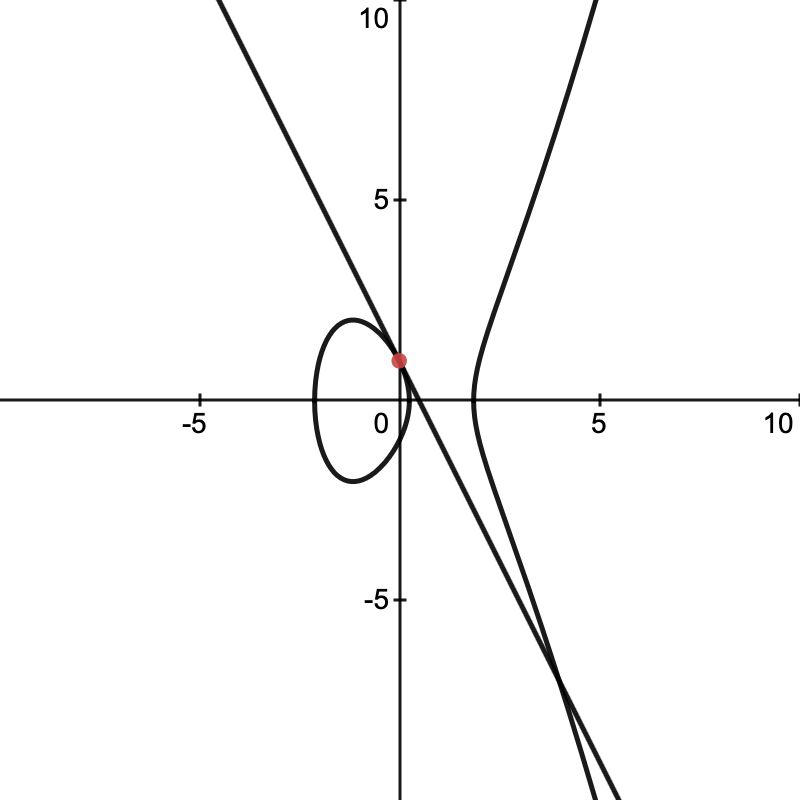
\includegraphics[width=0.5\textwidth]{fig1}
	\caption{Tangent line to a curve}
\end{figure}

A larger class of curves can be described by the equation $F(x,y) = 0$. Such a representation is called an \textbf{implicit} function. Figure 1 depicts the curve of the implicit function $y^2-x^3+4x-1 = 0$ along with its tangent line $y = -2x+1$ tangent at the point $(0,1)$.

\section{Implicit Derivative of $y^2-x^3+4x-1 = 0$}
In order to compute the derivative of an implicit function, think of the variable $y$ as an explicit function of $x$. To do this, rewrite the implicit function as $F(x,y(x)) = 0$. Using $y^2-x^3+4x-1 = 0$ as an example, the equation becomes \[y(x)^2-x^3+4x-1=0\] Next, take derivatives with respect to $x$ making sure to use the chain rule when dealing with the $y$ variable. \[2y(x)y'(x)-3x^2+4 = 0\] This final equation contains $x$ and $y$ variables as well as the derivative $y'(x)$. The final step is to solve the equation for $y'(x)$ in terms of both $x$ and $y$. \[y'(x) = \frac{3x^2-4}{2y(x)}\] We can drop the function notation with the $y$ and $y'$ variables to obtain the implicit derivative \[y' = \frac{3x^2-4}{2y}\] Observe that we need to know both the $x$ and $y$ coordinates in order to find the slope of the tangent line. Using the point $(0,1)$, the slope of the tangent line is given by $y'|_{(0,1)} = -2$, and the equation of the tangent line is $y = -2x+1$. \textbf{In summary},
\begin{itemize}
	\item Replace $y$ with $y(x)$
	\item Take derivatives of both sides of the equation. Remember to use the chain rule to evaluate derivatives of terms containing $y(x)$.
	\item Solve for $y'(x)$ in terms of $x$ and $y$
	\item Plug in $x$ and $y$ coordinates to get slope of tangent line.
\end{itemize}

\section{Implicit Derivative of $x^4 = 2(x^2-y^2)$}
Replace $y$ with $y(x)$. \[x^4 = 2(x^2-y(x)^2)\] Take the derivative of both sides. \[4x^3 = 4x+4y(x)y'(x)\] Solve for $y'(x)$. \[y'(x) = \frac{x-x^3}{y(x)}\] Drop the function notation, \[y' = \frac{x-x^3}{y}\] Oftentimes, the implicit derivative will be given as a fraction. This form can be useful for identifying vertical tangent lines and horizontal tangent lines. \textbf{Horizontal tangent lines occur when the numerator of the derivative is 0 and the denominator is nonzero.}

\begin{figure}[h]
	\centering
	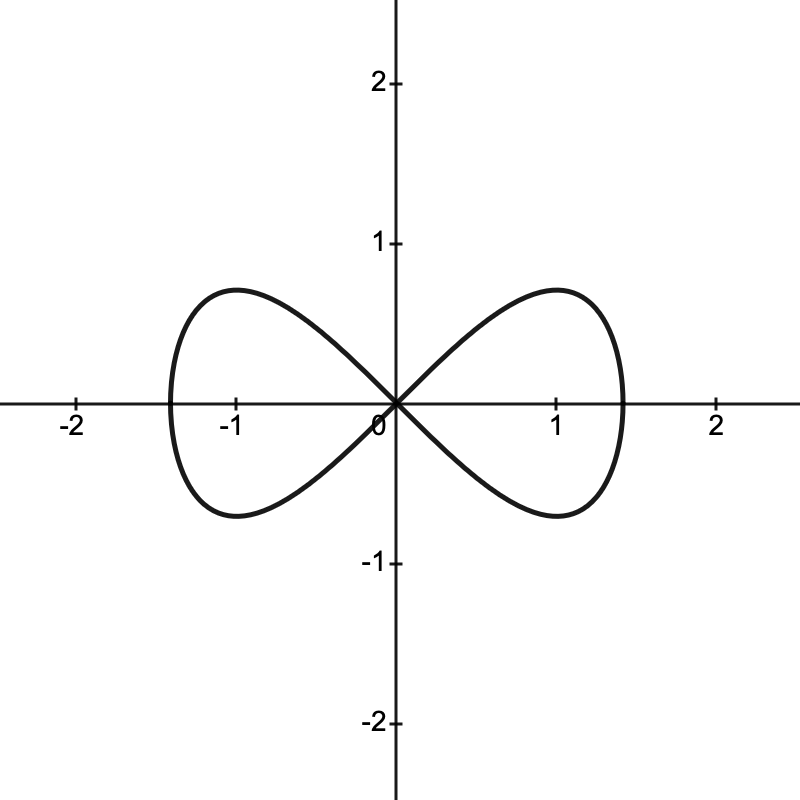
\includegraphics[width=0.5\textwidth]{fig2}
	\caption{Graph of $x^4 = 2(x^2-y^2)$}
\end{figure}

\noindent Setting the numerator of this curve to 0 yields the equation $x-x^3 = 0$ with solutions $x = -1, 0, 1$. Setting $x$ equal to each of these solutions for the original curve $x^4 = 2(x^2-y^2)$ yields the points $(0,0)$, $(1,\frac{\sqrt{2}}{2})$, $(1,-\frac{\sqrt{2}}{2})$, $(-1,\frac{\sqrt{2}}{2})$, $(-1,-\frac{\sqrt{2}}{2})$. Observe that the point $(0,0)$ will yield $\frac{0}{0}$ when plugged into the derivative. This does not correspond to a horizontal tangent line as seen in Figure 2.

\textbf{Vertical tangent lines occur when the denominator of the derivative is 0 and the numerator is nonzero.}  Setting the denominator to 0 yields the equation $y=0$. Plugging this in to the original curve yields the points $(\sqrt{2},0)$, $(-\sqrt{2},0)$, and $(0,0)$. Again, the point $(0,0)$ will yield $\frac{0}{0}$ when plugged into the derivative and will not correspond to a vertical tangent line.


\section{Second Order Implicit Derivatives}
Consider the implicit function $x^2-y^2 = 1$. Applying the method outlined in section 2, \[y' = \frac{x}{y}\] We can repeat this process again to find the second derivative $y''(x)$. Take derivatives of both sides \[y'' = \frac{y-xy'}{y^2}\] Note that the \textbf{chain rule was not used when taking the derivative of $y'(x)$} since that is the definition of the second derivative. To eliminate $y'$ from the right side of the equation \textbf{use the equation for $y'$ solved in terms of $x$ and $y$.} \[y'' = \frac{y-x(x/y)}{y^2} = \frac{y^2-x^2}{y^3}\] At the point $(2,\sqrt{3})$ on the curve, \[y''|_{(2,\sqrt{3})} = -3^{3/2} \approx -5.196\]
\end{document}